\section{IoTDSL}
\label{sec:IoTDSL}

Based on the challenges identified in section~\ref{sec:Motivation}, we now introduce \IOTDSL, our \DSL devoted to facilitate the high-level manipulation of \IOT systems. At the heart of \IOTDSL are two governing principles. First, we promote a clean separation of concerns for all aspects the \DSL has to handle, by specifying three sub-languages. We believe this approach to be scalable, and to support independent evolutions of each concern without impacting the other aspects, since those aspects are composed through well-defined interfaces. Second, our \DSL relies on events, a natural paradigm for specifying various models of interactions that is widely used in embedded and critical systems, and where a clear separation between the system and its environment is performed, further empowering the separation of concerns. Despite its early stage of development, \IOTDSL shows its ability to capture the definition of small-scale \IOT systems appropriately.

Building a well-calibrated \DSL is known to be difficult and error-prone. It usually requires a broad expertise of the domain under consideration before a consensus emerges on the domain's key concepts and how to effectively represent them. Fortunately, \MDE technologies operated substantial breakthrough over the past decade, allowing language designers to define their own \DSL structures and user interfaces more easily. Adopting such a trend, we have built an early prototype for our \DSL under \textit{GeMoC} \cite{bousse-16}, a \MDE framework that supports both visual and textual representations as concrete syntaxes and maintains a full synchronisation between them. Since we are at early development stage, only a textual syntax is currently available to modellers, but other syntaxes, even graphical ones, can be added smoothly thanks to \textit{GeMoc}.

To illustrate our proposal, we start by depicting the language's metamodel where we highlight its main features. We then illustrate the available constructs in \IOTDSL with the hypothetical scenario presented in section~\ref{sec:Motivation}.

\subsection{Type Definition}
\label{sec:IoTDSL-Type}

In this section, we define \IOT devices' types, \textit{i.e.} which capabilities are available to the users in terms of getting information from the environment, \textit{a.k.a.} sensing, and operating on the environment, \textit{a.k.a} actuating. In our framework, type definitions either come from an advanced user who is able to reason properly about a particular device and extract the relevant information, or from a pre-existing devices database, either being a repository the system is connected to, or a library of \textit{devices-off-the-shelf}. 

\begin{figure*}%
  \centering  
  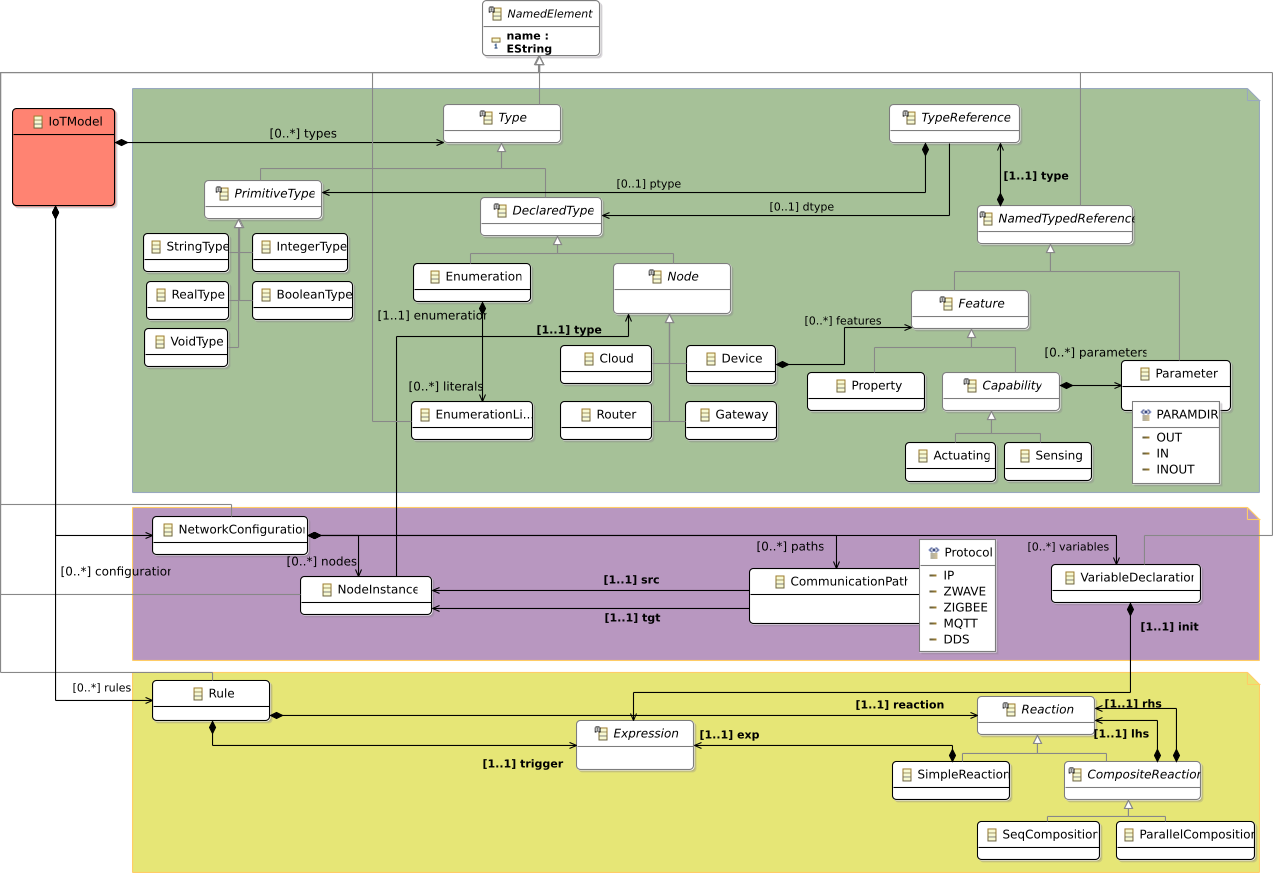
\includegraphics[width=.92\linewidth]{IoTDevice-MM.png}%
  \caption{Metamodel of \IOTDSL, separated in three concerns: \emph{Type Definition} captures devices' capabilities (top green part), \emph{Network Configuration} details how device instances are connected to each others (middle purple part), \emph{Business Rules} defines the functionalities expected from the IoT installation (bottom yellow part).}%
  \label{fig:IoTDevice-MM}%
\end{figure*}

The concepts dedicated to type definition are shown in Figure~\ref{fig:IoTDevice-MM} (green background). This part is similar to the notion of \textsf{Classifier} in \textsc{Mof}-like languages: a \textsf{Type} is either a \textsf{PrimitiveType}, or a user-defined \textsf{DeclaredType}. We distinguish between general \textsf{Gateway}s, which centralise information and processing, and \textsf{Node}s deployed in the environment, having capabilities and transferring data to \textsf{Gateway}s. A \textsf{Capability} is basically a \textsc{Mof}-like operation with a list of \textsf{Parameter}s that either captures data from the environment, or acts on it. A \textsf{Node} can mix both kinds of capabilities, allowing us to represent complex behaviour in a uniform fashion. Also note that \textsf{Node}s are \textsf{Type}s themselves such that their references may be passed a \textsf{Capability} parameters for the purpose of dynamic discovery across devices.

%For now, types are defined in specific files that can be imported and combined easily within \IOT specifications. We plan to propose a graphical interface to facilitate the browsing and integration of library components into \IOT systems.

In Listing~\ref{lis:RE-TypeDeclarations}, we illustrates how devices are declared in \IOTDSL. Each device is introduced by the keyword \textsf{device}, it has a name and capabilities that correspond to reporting events (\textsf{sensing}) or operating over the environment (\textsf{actuating}). In this listing, we declare the capabilities of all devices presented in Figure~\ref{fig:scenario}.

\begin{table}
	\begin{minipage}[b]{.45\textwidth }%
		\begin{lstlisting}[language=iotdsl]	
gateway Middleware
device DoorDetector {
	sensing opened()
	sensing closed()
}
device MotionDetector {
	sensing moving()
}
device ToggleSwitch {
	sensing toggle();
}
		\end{lstlisting}
	\end{minipage}\hfill%
	\begin{minipage}[b]{.45\textwidth}
		\begin{lstlisting}[language=iotdsl, firstnumber=12]
device LightSensor {
	sensing light(out isLight:Boolean)
}
device LightBulb {
	sensing lightOn()
	actuating on()
	actuating off()
}	
device Alarm {
	actuating sound()
}
    \end{lstlisting}
	\end{minipage}
\captionof{lstlisting}{Type declarations in \IOTDSL: \textsf{sensing} or \textsf{actuating} capabilities as high-level events.}
\label{lis:RE-TypeDeclarations}
\end{table}

A special device, introduced with the keyword \textsf{gateway} will be in charge of centralising data from all devices connected to it, as we will show in Section \ref{sec:IoTDSL-NetworkConfiguration}. This device will be responsible of the event orchestration and will host the \CEP engine that embeds the implementation of the business rules. Also note that the above model is the \textit{user-defined} part of \IOTDSL. In the background, abstract events attached to all devices will need to be mapped to concrete low-level APIs events using a dedicated mapping language that is out of the scope of this paper.

\subsection{Network Configuration}
\label{sec:IoTDSL-NetworkConfiguration}

The configuration constructs of \IOTDSL are specified in the purple-part of Figure~\ref{fig:IoTDevice-MM}. A concrete device is represented by a \textsf{NodeInstance} and is typed by an abstract \textsf{Node}, \textit{e.g.} a \textsf{Device} or a \textsf{Gateway} specified at the typing level. Instances may communicate with other \IOT devices through predefined \textsf{CommunicationPath}s. Such paths define, among others, one or more protocols used to interact. We actually rely on existing platforms, such as OpenRemote\footnote{\url{http://www.openremote.org}} or SmartThings\footnote{\url{https://www.smartthings.com/}} to handle the intricate details of the protocols since such details are, from an end-user point of view, technical aspects rather than essential matters of the configuration itself. By knowing which protocols are used between each pair of devices, we can automatically perform data conversion in the proper format required by the protocols: most of those protocols are already implemented in \textit{General-Purpose Programming Languages} (\textsc{Gpl}s), like Java or C.

Listing~\ref{lis:RE-Network} shows an instantiation as well as the connection that conforms to the types given in Listing~\ref{lis:RE-TypeDeclarations} and the configuration presented in Figure~\ref{fig:scenario}.
	
	
\begin{table}
	\begin{minipage}[b]{.45\textwidth }%
		\begin{lstlisting}[language=iotdsl]	
configuration SmartHouse {
	node middle   		   : Middleware
	node alarm					 : Alarm
	node toggle          : ToggleSwitch
	node frontDoor			 : DoorDetector
	node parentDoor			 : DoorDetector
	node childDoor			 : DoorDetector
	node balconyDoor 		 : DoorDetector
	node outLight				 : LightSensor
	node livingLight		 : LightSensor
	node livingBulb			 : LightBulb
	node bathroomBulb    : LightBulb
	node foyerBulb       : LightBulb
	node balconyMotion	 : MotionDetector
	node foyerMotion  	 : MotionDetector
	node hallMotion	     : MotionDetector
		\end{lstlisting}
	\end{minipage}\hfill%
	\begin{minipage}[b]{.45\textwidth}
		\begin{lstlisting}[language=iotdsl, firstnumber=17]
	from alarm			   to middle via IP
	from frontDoor 	   to middle via IP
	from parentDoor    to middle via IP
	from childDoor     to middle via IP
	from balconyDoor   to middle via IP
	from outLight      to middle via IP
	from livingLight   to middle via IP
	from livingBulb    to middle via IP
	from bathroomBulb  to middle via IP
	from corridorBulb  to middle via IP
	from balconyMotion to middle via IP
	from frontMotion   to middle via IP
	from hallMotion    to middle via IP
}
		\end{lstlisting}
		\vspace*{.3cm}
	\end{minipage}
	\captionof{lstlisting}{Network Configuration in \IOTDSL for our smart house.}
	\label{lis:RE-Network}
\end{table}
	
A specific device is considered as an instance of a defined type such that particular devices with the same set of capabilities may be distinguished via identifiable unique references. Communications are purely declarative and only mention the protocol type (introduced by the \textsf{via} keyword). In our example, we simply decided to use an \textsf{IP} protocol for all bindings. Note that a similar mapping process that the one described at the end of Section~\ref{sec:IoTDSL-Type} is required to reify abstract connections between \textsf{NodeInstances} to physical ports and protocols, but again, these mapping statements are outside of the scope of this paper. 

\subsection{Business Rules}
\label{sec:IoTDSL-BusinessRules}

Business rules are the core of the manipulation of \IOT systems and compose the third part of \IOTDSL as detailed in the bottom yellow part of Figure~\ref{fig:IoTDevice-MM}. This last sub-language relies on an event-based framework that allows to specify a set of \textsf{Rule}s expressing the many functionalities an end-user wants to achieve in his/her concrete configuration. 

In \IOTDSL, a rule is identified by the keyword \textsf{rule} followed by an unique identifier and its body is of the form << \texttt{\textbf{\color{codeviolet}{when}} (trigger) \textbf{\color{codeviolet}{do}} \{ reaction \}} >>, where the \textsf{trigger} specifies a boolean condition under which given \textsf{reaction} must be triggered. Rules' \textsf{trigger}s are cyclically evaluated against the surrounding environment and a \textsf{reaction} defines a sequential or parallel combination of capabilities, enabling to sort actions by, or require data from some identifiable devices. Inside the \textsf{trigger}, users typically check events to evaluate their presences, but as we will see in the following examples, they are also able to check on their absence or returned values. A typical \textsf{reaction} may be to switch on all lights in a house, or only the ones of a certain type by sending new events.

For now, our approach is purely middleware-oriented: rules are gathered and evaluated into a single gateway. For efficiency and resource consumption reasons, we are also exploring how to automatically identify parts of the business logic that can be exported to advanced nodes with sufficient processing and power resources in order to lower network and gateway overuses.

We now illustrate how our smart house scenario presented in Section \ref{sec:Motivation} can be translated into business rules in \IOTDSL with the devices' definitions detailed in Listings~\ref{lis:RE-TypeDeclarations} and \ref{lis:RE-Network}. We identified three different situations to depict the usage of business rules and highlight the main assets of \IOTDSL.

\subsubsection*{Light on when coming home}

When Alice gets home (and thus opens the front door), she wants the lights to be automatically switched on in the foyer and in the living room.

\begin{lstlisting}[language=iotdsl,label=lis:home-rule,caption=\IOTDSL business rule to switch on the lights when coming home]
rule SwitchLightsWhenEnter:
  when (frontDoor.opened() and after foyerMotion.moving()) do {
    foyerBulb.on()
    livingBulb.on()
  }
\end{lstlisting}

As we are dealing with concurrent events, we introduce two special operators on top of common boolean operators, called \textsf{before} and \textsf{after}. With these event modifiers we are able to check that two events connected by a binary operator (an \texttt{and} in this particular example) appear in a reasonable time window. In the above rule, the \texttt{frontDoor} must be opened and \textit{quasi subsequently} followed by a movement detection by the \texttt{foyerMotion}.

One or more events, declared in a rather imperative way may be triggered from a rule. The concrete execution semantics is left to the user, where in some cases, all events will be produced asynchronously or simultaneously, where in other they will be produced sequentially. This freedom in the language is meant to cover any execution semantics, especially because this semantics is often domain-specific and depends on technical details our end users probably do not want to deal with at that level of abstraction.

\subsubsection*{Light on when child wakes up at night}
	
When Alice's child wakes up at night, she would like to have the light in the bathroom to be switched on to prevent her from falling or injuring herself. Analogously, she wants the light to be switched off when she gets back to sleep afterwards.

\begin{lstlisting}[language=iotdsl,label=lis:night-rule,caption=\IOTDSL business rules to switch on\//off the lights at night]
rule SwitchBathroomLightOnAtNight:	
  when (outLight.light(l) == false and livingLight.light(l) == false 
  		and (childDoor.opened() and after hallMotion.moving())) do {
  	bathroomBulb.on()
  }
  
rule SwitchBathroomLightOffAtNight:	
	when (not hallMotion.moving() within 3 min from childDoor.closed() 
			and outLight.light(l) == false) do {
		bathroomBulb.off()
	}
\end{lstlisting}

The first rule expresses that, at night, when both \texttt{LightSensor} are sending \texttt{false} values and when Alice's child opens her door \textit{immediately} followed by some movements in the hall, the light in the bathroom is switched on. As the \texttt{LightSensor.light()} events are typed events sending boolean values, we have to evaluate their values with the parameter \texttt{l} implicitly resolved as the event argument. We also note that at line 3, we must use parenthesis because the \textsf{after} modifier needs to know what (set of) events must precede the other(s) event(s) on the right hand side. 

The second rule in Listing~\ref{lis:night-rule} checks on the absence of an event \textsf{within} a given time frame after (\textit{i.e.} \textsf{from}) another event has been detected. In this rule, we state that when no more movement have been detected in the hall for three minutes after the door of the child's room has been closed, the light in the bathroom must be switched off. In \IOTDSL, users are then able to check on the absence of an event within a time frame of their choice (with a set of predefined time units). It is worth noting that the \textsf{not} qualifiers is only used to check on the absence of an event, where the \texttt{outLight.light(l) == false} checks on the return value of the event. We could have had an event returning \textsf{integer} values like \texttt{0} or \texttt{1} so the boolean expression would have been \texttt{outLight.light(l) == 0}.

\subsubsection*{Child on balcony without surveillance}
	
There is a critical situation when Alice's child goes onto the balcony without supervision. To that end, Alice has placed a switch button that an adult has to press when going on the balcony. If the toggle switch is not pressed within 3 sec after someone gets onto the balcony, the alarm must ring.

\begin{lstlisting}[language=iotdsl,label=lis:balcony-rule,caption=\IOTDSL business rules ring the alarm when Alice's child alone on balcony]
rule AlarmWhenChildOnBalcony:	
  when (not toggle.toggle() within 3 sec from 
  		(balconyDoor.opened() and after balconyMotion.moving())) do {
    alarm.sound()
  }
\end{lstlisting}

In other words, the above rule states that after the door of the balcony has been opened and any movement has been detected on the balcony, but no toggle button has been pressed in the next 3 seconds, the alarm must ring. This last rule is somewhat similar to the ones in Listing~\ref{lis:night-rule} except that we combine the absence of an event in a time frame directly followed by the detection of other events in a sequential or in quasi simultaneity. In \IOTDSL, users are then able to fully describe a sequential execution of events, \textit{i.e} a complete business workflow, that must be checked before triggering some \textsf{reaction}.

